\documentclass[a4paper,11pt,twoside]{article}
%\documentclass[a4paper,11pt,twoside,se]{article}

\usepackage{UmUStudentReport}
\usepackage{verbatim}   % Multi-line comments using \begin{comment}
\usepackage{courier}    % Nicer fonts are used. (not necessary)
\usepackage{pslatex}    % Also nicer fonts. (not necessary)
\usepackage[pdftex]{graphicx}   % allows including pdf figures
\usepackage{listings}
\usepackage{pgf-umlcd}
\usepackage{blindtext}
\usepackage{rotating}
\usepackage{enumitem}
%\usepackage{lmodern}   % Optional fonts. (not necessary)
%\usepackage{tabularx}
%\usepackage{microtype} % Provides some typographic improvements over default settings
%\usepackage{placeins}  % For aligning images with \FloatBarrier
%\usepackage{booktabs}  % For nice-looking tables
%\usepackage{titlesec}  % More granular control of sections.

% DOCUMENT INFO
% =============
\department{Department of Computing Science}
\coursename{Development of Mobile Appliations 7.5 p}
\coursecode{5DV155}
\title{`Mealpricer' - Free of Choice App Project}
\author{Lorenz Gerber ({\tt{dv15lgr@cs.umu.se}} {\tt{lozger03@student.umu.se}})}
\date{2017-08-21}
%\revisiondate{2016-01-18}
\instructor{Johan Eliasson / Jonathan Westin}


% DOCUMENT SETTINGS
% =================
\bibliographystyle{plain}
%\bibliographystyle{ieee}
\pagestyle{fancy}
\raggedbottom
\setcounter{secnumdepth}{2}
\setcounter{tocdepth}{2}
%\graphicspath{{images/}}   %Path for images

\usepackage{float}
\floatstyle{ruled}
\newfloat{listing}{thp}{lop}
\floatname{listing}{Listing}



% DEFINES
% =======
%\newcommand{\mycommand}{<latex code>}

% DOCUMENT
% ========
\begin{document}
\lstset{language=C}
\maketitle
\thispagestyle{empty}
\newpage
\tableofcontents
\thispagestyle{empty}
\newpage

\clearpage
\pagenumbering{arabic}

\section{Introduction}
The aim was to come up with a good idea for a reasonable sized mobile application
that should then be implemented. Reasonable size here was that implementation should
be possible in about 60 hours of work (1.5 week).

During the course, there were some propositions of possible applications where one
was a cooking recipt app with shopping list functionality. I like to cook and I am
usually on a tight budget. Further, I actually like to guess or calculate the price
of all kind of stuff I see around me. Hence, from the cooking receipt application I got
inspired to develop `Mealpricer', an app to calculate the fractional costs of meals.

Generally, wile pondering about potential projects, I was convinced that I did not
want to implement a game as this would involve mostly general java programming. My
aim was to find a project that would give me the possibility to improve on my
general crafts for navigating the android framework. In my opinion, the most typical
mobile application is data centric. It presents some sort of data in lists. Currently,
to make a professional looking android app, I think it is indispensable to master the
elements of material design. Therefore, another aim for me was to incorparate
as much material design as possible in my project. So far, I have not spent much
time with GUI programming in general, there I wanted to develop more in this field.


\section{General Description and Target Group}
The envisioned and implemented android app with the name `Mealpricer' is
targeted towards indviduals that are looking for a tool to quick and easily determine
the fractional cost of a specific meal.

I checked out the Google Play Store for similar apps. There were a few with a
smiliar idea. There I also realized the potential behind the
concept: Calculating fractional costs of a meal from bulk ingredient prices and
ingredient amounts is actually a very common application for restaurants to price
their meals.

So besides individuals, I think this application could make a good tool for
food and catering professionals to quickly recalculate meal prices while
shopping for ingredients.

\section{PlayStore Description}
\textit{MealPricer is an application that helps you to keep track of how much individual
meals that you prepare cost. Whether you are a student on a tight budget or a
restaurant owner that wants to calculate the fractional costs of his offerings
from bulk products, MealPricer will help you in the most simple way to keep track
of it.}

\section{Target Course Grade}
I aim for a 'VG'. Below follows some reasoning around it.

I have spent quite a bit more time on the app than the indicated
target of 60 hours. I am aware that for a senior android developer, such an
app could be developed in a fraction of that time. However, I think it is
also understood that this is an introduction course to the android framework, hence
additional time is justified.

Generally, I am pretty happy with the result of my application. I am aware that
the app has a rather simple concept with an easy to implement data model. But this
was also by purpose as mentioned earlier: My aim was to spend as much time as
possible with actual android framwork programming and not general Java. I think that
the final product looks appealing and can be used practically. I spent quite some
time on drafting the initial flow of the app and looking up which concepts of
material design that would make for a good user experience.



\section{Aspects on Security and Ethics}
MealPricer in it's current form is both from a security and ethics point of
view rather unproblematic. In terms of security, all the data is stored only
locally, withing the application directory. There is currently no possiblity
from another app to make use of the MealPricer data or to use a service from
MealPricer that would give access to user data.
One Issue, that is currently solved rather clumsy are the photos, which are
stored at full size. This should be either adjusted to store a scaled, less
storage intense version, or to at least inform the user about it. In a more
advanced version of MealPricer, photos could be stored in a already accepted
thirdparty app such as Google Photos, or the images could be stored in the
cloud, if MealPricer would get launch as a more advanced service with own
backend servers. Such a service would need more detailed considerations regarding
both security but also ethics.

In general, the data does not seem to be of very privacy sensitive type, however,
if collected in a cloud service, MealPricer data from a large userbase
could become valuable to marketing or food related services and companies. As such,
ethical handling of user privacy could become an issue.


\section{User Guide - How To}
\subsection{General Intro}
MealPricer is used to calculate the fractional cost of a meal from bulk
ingredient prices. To start using MealPricer, you should first enter a number
of products that you use for your meals.

\subsection{Step by step}
Mealpricer opens automatically on the main page, `Meals'. If you open MealPricer
for the first time, there will be no entries. The main view of MealPricer
consists however of two views that are organized side by side as tabs. By
swiping from right to left, you activate the product tab. Here you can press
the pink colored `add'  button in the lower right corner to start entering a new
product. First you enter the name in the upcoming dialog. You can later stil
modify the name.


\begin{figure}

  \centering
    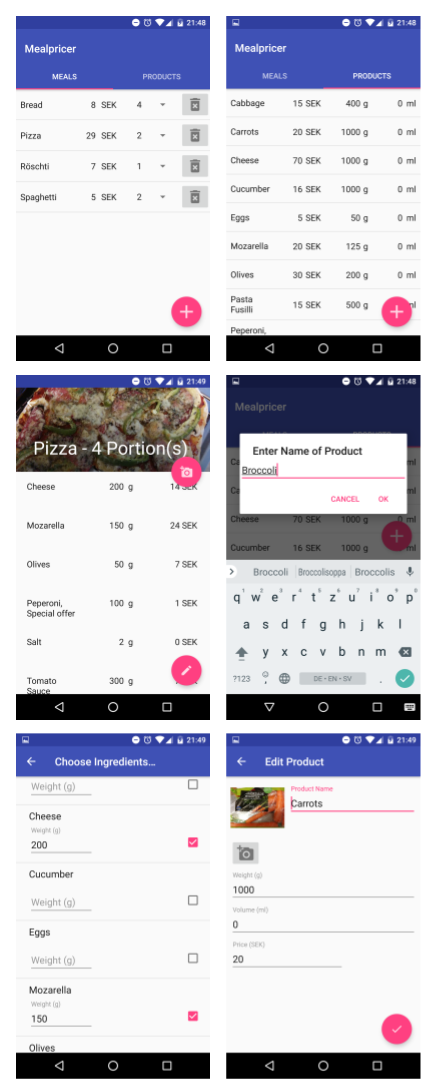
\includegraphics[width=0.7\textwidth]{images/screenshots.png}
    \caption{A picture of a gull.}
    \label{fig:screenshots}
\end{figure}

After pressing `OK' you enter the `Product Edit' screen where
you enter the requested info about amount and price. On pressing the button with
the camera icon, you can take a photo of your product. All prices are calculated
either by volume or by weight, hence, this you should enter either of them together
with the corresponding price. For convenience with some products, it can make
sense to enter both weight and volume information. Mealpricer of course has no
possibility whether the values correspond to the indicated price. When you have
finished entering the product details, you get back to the product list view
either by the ok tick mark button in the lower right or by the top menu `up'
arrow. To edit existing products, you can tap the product in the list which
will bring you back to the edit view.

When you have entered enough products to compose your meal, you can swipe back
to the meal tab. There you press the `add' button in the lower right corner.
In the dialog, you can choose the name of the meal and for how many portions
you want to enter the indgredients. On Pressing ok, you come to the detail
view of an individual meal. This view is currently empty, until you have chosen
the ingredients which you do by pressing the `edit' button in the lower right
corner. The ingredient edit screen allows you to choose which ingredients and
how much of them are used for the meal. When you are finished, you press the
`up' arrow in the menubar. Now you can see all the fractional costs for all
ingredients of the meal. With `pink' camera button at the top of the screen,
you can take a photo of the meal that will then show up in the extensible
menu bar. The `up' menu button brings you back to the meal list. Here you can
now see the total price of the meal. You can also choose to recalculate the
price for a different portion size by tapping the spinner next to the price
indication. Meals can be removed by pressing the waste bin icon in the right
end of each meal list entry.



\section{Application Architecture}
\subsection{General Structure and Flow}
After the idea of Mealpricer was born, it was decided how many views
would be needed and in which sequence it would make sense to arrange them. An
early design draft is shown in figure \ref{fig:design_draft}. There it can already be seen that the
main application models would be meals, products and ingredients. The base view
of the application was chosen to consist of two pages that are connected as
tabs. Technically, this was implemented using an activity that hosts two framgents
using a pager adapter. The fragments themselves both host a recycler list view
for each the meals and the products. Both these recycler view implement list
item touch navigation: On touching a list item, the user is brought to the next
activity, either the MealDetail activity or the ProductDetail activity.

\begin{figure}

  \centering
    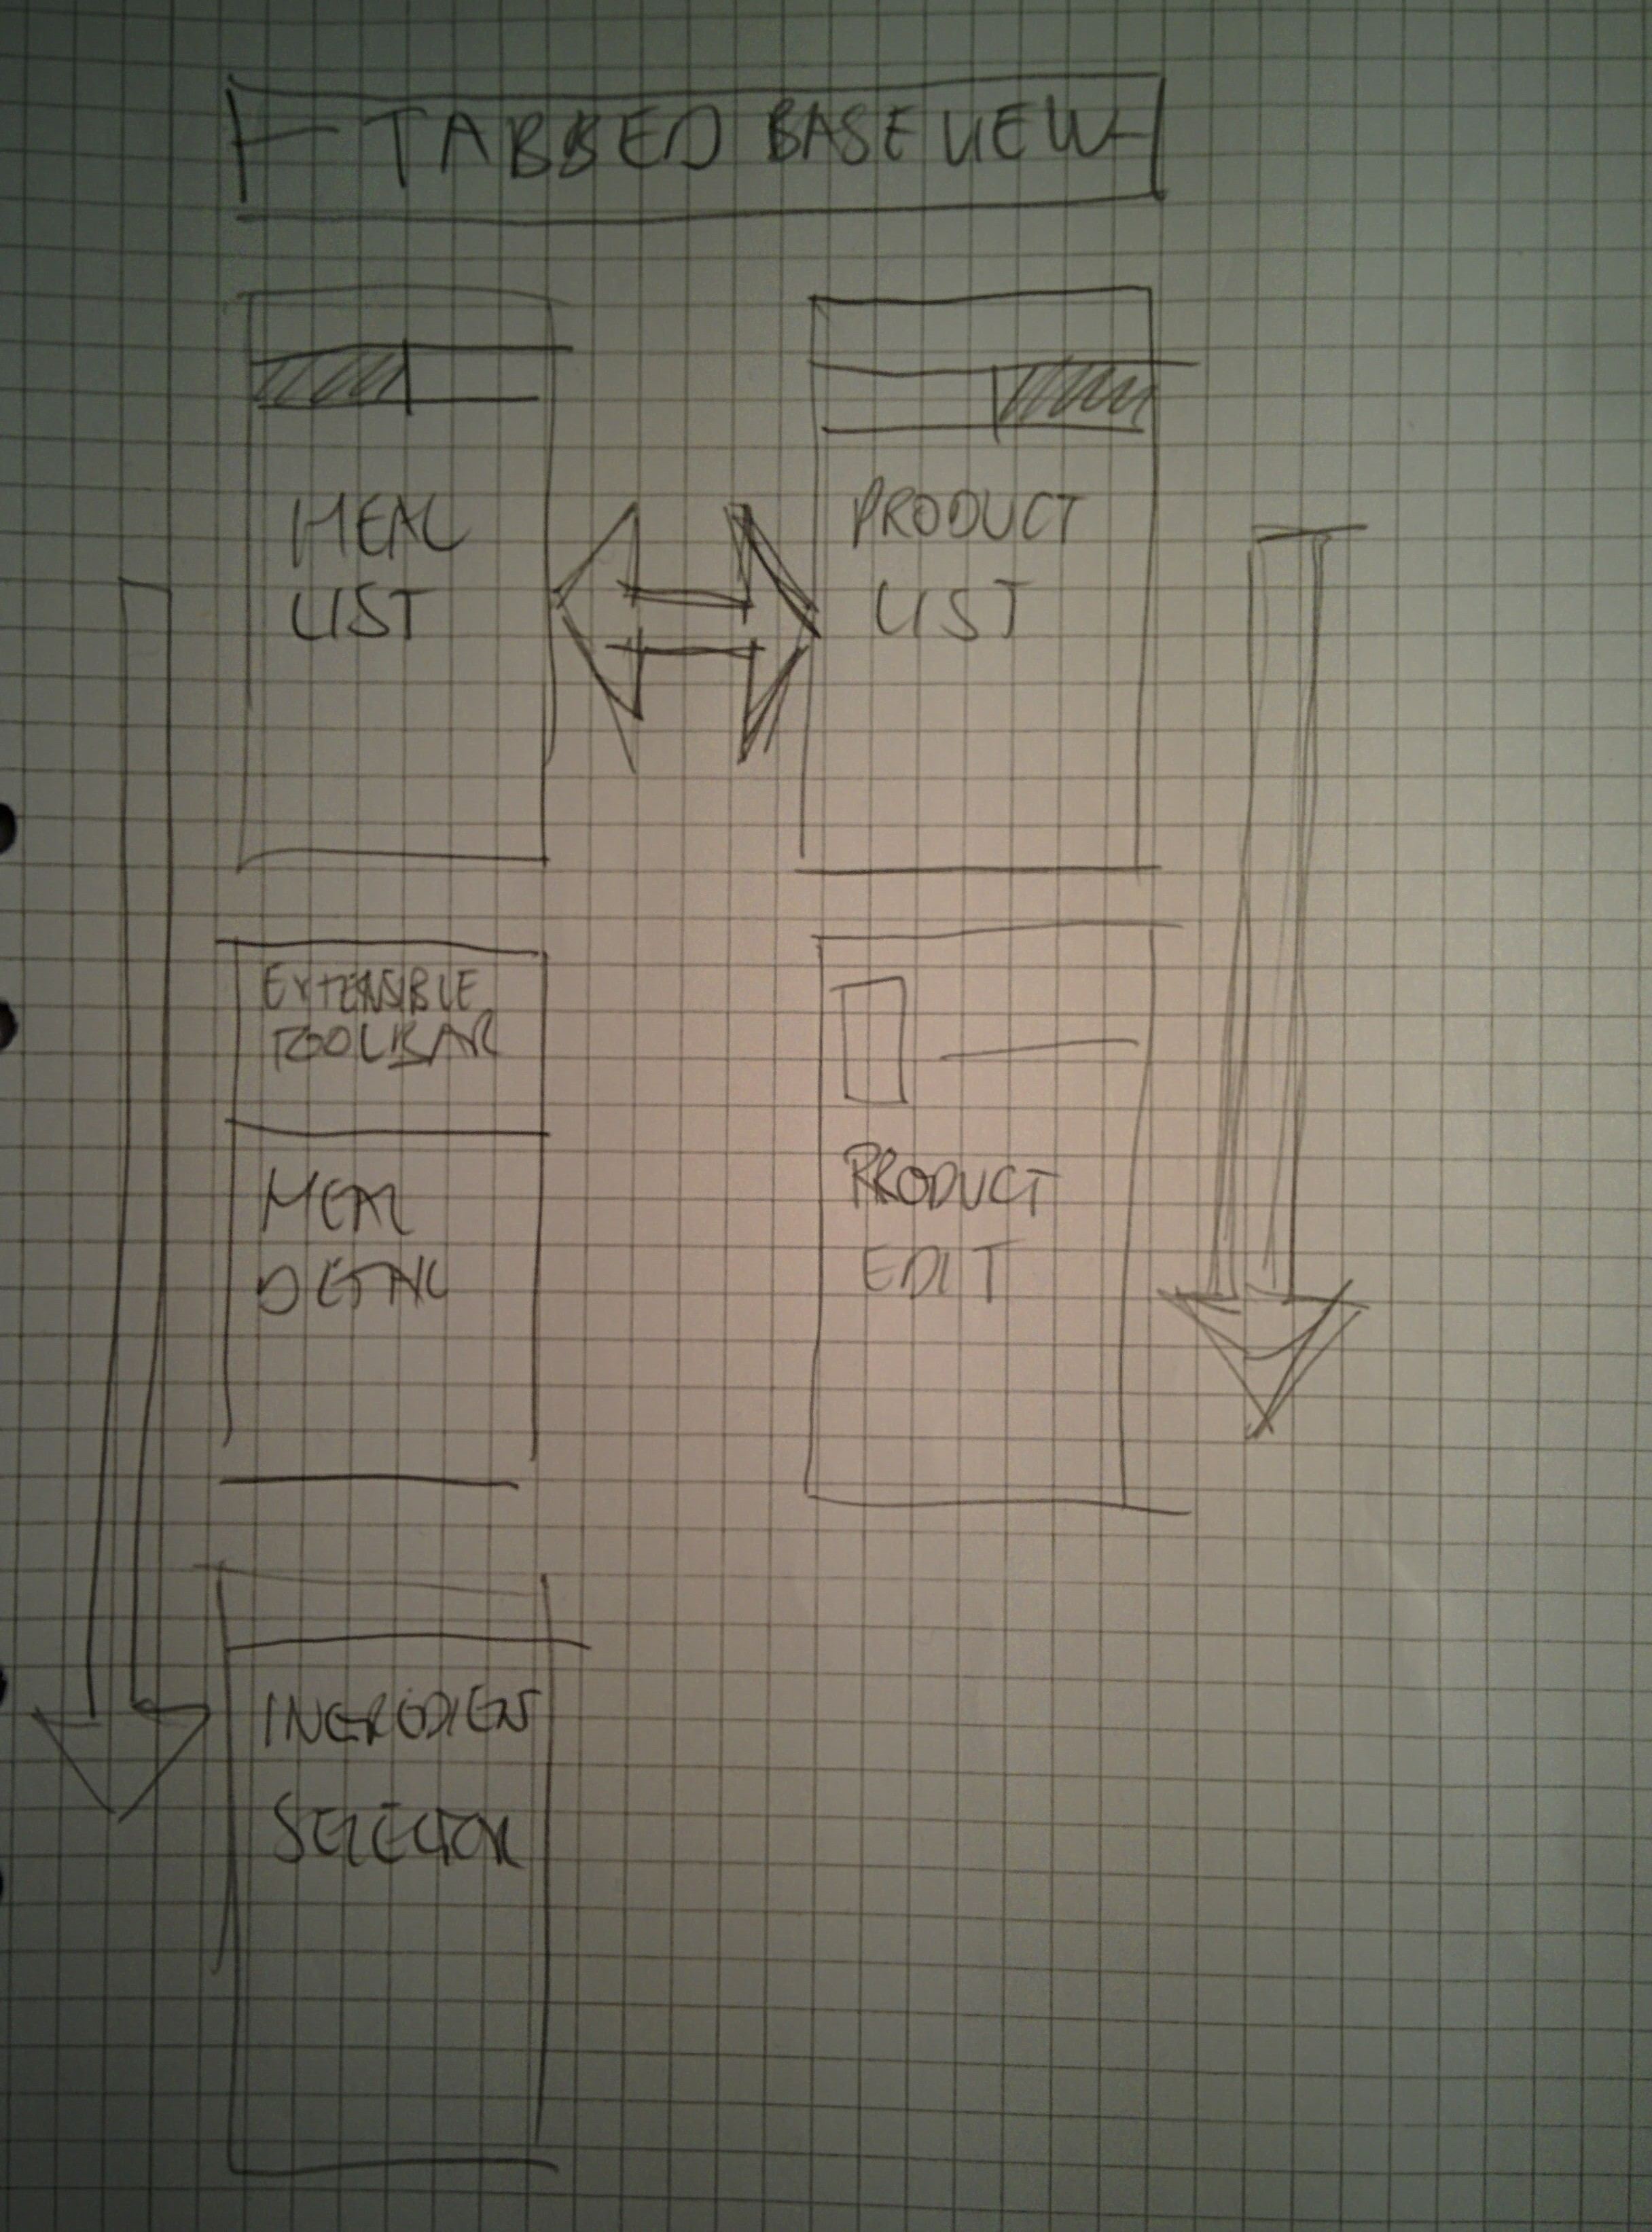
\includegraphics[width=\textwidth]{images/design_draft.jpg}
    \caption{A picture of a gull.}
    \label{fig:design_draft}
\end{figure}


If the user wants to add new list elements, in both the meal and product list an
alert dialog is shown that allows the user to chose a name for the new meal or
product and in the case of the meal, also the portion. The alert dialog step allows
to open the respective edit activity directly with an element that exists already
in the database. This has certain advantages to keep the data flow in the application
as simple and consistent as possible.

While the meal and product list shared one Activty to handle the tabs, the detail
views have each their own activity. The whole application makes active use of
material design elements such as floating action buttons, collapsing toolbars
and tabbed screens. Many of these patterns can be implemented using templates. For an
experienced android programmer, these should speed up development significantly.
When using them first time however, there was usually quite some confusion until
the general concept was grasped.

The main element of the application can be said to be recycler view lists in
several variations. The most complex is the one where ingredients can be chosen
for an idividual meal. The implementation of widgets with interconnected listeners
was not obvious from the beginning. Some details on it's implementation will be
given further down as a special topic.

The application uses a database to store all application data expect the binary
photo data. The photos are currently stored freely in the application directory
using the unique id's of the meal respective the product. When a corresponding
element is deleted in the database, a separate routine will check whether there
exists a photo which in turn will also be removed. As such, the application
should keep it's space clean and tidy.

To take photos an implicit intent is used. The photos are currently stored at
full size. This is probably not the best idea, however, the idea for a future
version would be to implement a simple web backend that stores the user data.

Photo's are shown in two places. Once they have to be only scaled, while in the
other place, as background of the `Flexible Space with Image - Collapsible Toolbar'
pattern they have to be both scaled and cropped. More details on this will also be
provided as a special topic further down.

Generally, the application model of MealPrcer is very simple. However, despite of
it's simplicity, there were already a number of concerns to make the user
experience consistent and logical throughout the whole application. There are for
example the issues what should happen if a user attempts to delete a product that
is still part of (a) meal(s). For ingredients, the same case was a simple choice
as it was decided to implement the ingredients table with references to the
unique identifiers of both meals and products. Hence, when a meal get's deleted,
all of it's products can also be removed from the database. Currently, for the
products, it was simply chosen to not allow deletion! This might sound drastic,
however in an early stage of this' apps liftetime, it works out surprisingly
well. The solution was to keep the product completely editable, including the
name and photo. As such, unused products can simply be changed to a new one.

There were a number of such architectural design deciscions. Of course, not all
of them are the most elegant solution, however, it became clear quite soon during
implementation, that in 1.5 weeks, there would not be enough time to polish the
app as much as one would like to. There were several phases during implementation,
such as designing the data model, optimizing the UI layout etc. Each of these
development phases needed a substantial amount of time and needed as such
a compromise in how many details could be solved.

\section{Selected Discussion Topics}

\subsection{Embedding Fragments statically/dynamically in Activity}
Trying to use the provided templates for google material designed activities and
fragments, I run into the situation where fragments where by default embedded into
activities by instantiating them in XML. This works fine when the Activity/Fragment
combo in question does not need to obtain extras on creation. In many cases however,
for example when the Activity/Fragment combo represents the detail view after a
list activity, the ID of the chosen list item has to be obtained. Hence, the given
template code had to be modified for dynamic instantiation of the fragment from
within the activity.
During planning for the above modification, it was noted that there are at least
three single activity / single fragment views in the current application. According
to the example in the course book, this could make up for an `Abstract'
`SingleFragmentActivity' class. However, it was decided against this due to
implications on the material design elements: The Appbar and Floating Action Button
are kept in the activity, while the content layout is in the fragment. But the
three single fragment activities don't share exactly the same setup for appbar
and Floating Action Buttons. Hence another layer of abstraction would be needed that
would make things overly verbose.

\subsection{Deciding on the Persistance Model} It was chosen in the beginning to
store the application data in SQLite. In many cases, it was possible to store
the data into the database on UI orientation changes. In some cases however, for
example the position of the portion spinner in the meal list view, the data is
not stored in the database. After having implemented an initial version where
the spinner would always return to the portion that is stored along with the
corresponding ingredient amounts, UI testing led to the conclusion that the spinner
position should at least be persisted during orientation change. This was then
done by using extras. Hence, in some cases, the current application uses various
techniques to persist the data.

\subsection{Deciding on Ingredient Chooser UI}
The ingredient choose turned out to be the most complex UI item. Bascially it is
implemented as a recycler view that holds three widgets in each row. The EditText
widgets are used to enter the amount of the ingredient for either volume or weight.
A checkbox is used to include the ingredient in the meal. This will result in
persisiting the ingredient to the database when the view is left or also on
orientation changes.

In a initial implementation, all listeners (TextWatcher and onCheckedChange) were
attached during the `onBind' override of the ViewHolder. This was chosen as attaching
them during instantiation of the ViewHolder resulted in a firing the listeners
already while loading the ViewHolder initially with data. However, attaching `onBind'
eventually turned out to be even worse: While already the performance was much worse,
during a stress test with many elements, it was found that the ViewHolder was not
working correctly as dozens of listeners were attached without ever being removed.
This led to glitches and seemingly unpredictable wrong behaviour.
After reading a number of StackOverflow threads, the correct way was found where
listeners are attached during instantiation, but are deactivated during onBind.


\addcontentsline{toc}{section}{\refname}
%\bibliography{references}

\end{document}
